%=== Préambule ===========================================================

\documentclass{beamer}
\usepackage{pdfpages}
\usepackage{pdfpages}
\usepackage{braille}
%\usepackage[english]{babel}
%\usepackage[latin1]{inputenc}
%\usepackage[cyr]{aeguill}
\usepackage[english]{babel}
\usepackage{xspace}
\usepackage{pifont}
\usepackage{hyperref}
\usepackage{listings}
\usepackage{csquotes}
\usepackage{graphicx}
\usepackage{animate,media9} %,movie15}
\usepackage{wrapfig}
\usepackage{pdfpages}
\usepackage{tikz}
\usepackage{natbib}
\uselanguage{English}
\usepackage{fontawesome5}
\languagepath{English}
\setcounter{tocdepth}{1}
\usepackage{setspace}
\usepackage{amsmath}
\def\glasses{{\sffamily 
\leavevmode\rlap{%
\rotatebox[origin=tr]{125}{J}\kern1ex%  
\rotatebox[origin=tr]{125}{J}}% 
\rotatebox[origin=c]{-90}{D}%   
\rotatebox[origin=c]{-90}{D}}%
\def\ialy{\sffamily 
\resizebox{1ex}{1.5ex}{\reflectbox{\rotatebox[origin=]{75}{J}}}\kern-1pt%
\rlap{\tiny$\ ^\bullet\kern2.5pt^\bullet$ }%
\rotatebox[origin=c]{-90}{D}%   
\rotatebox[origin=c]{-90}{D}\kern-1pt%  
\resizebox{1ex}{1.5ex}{\rotatebox[origin=]{75}{J}}}}


\lstset{
  numbers=left,
  basicstyle=\tiny\ttfamily,      
  breaklines=true, 
  showtabs=false,
  showstringspaces=false,
}  

%=== Configuration de Beamer et du thème metropolis ======================
\usepackage{bbding}
\usetheme[background=light]{metropolis}
\usepackage[clock]{ifsym}

\definecolor{mLightBrown}{HTML}{000000}
\definecolor{black}{HTML}{000000}
\setbeamercolor{structure}{fg=black,bg=mLightBrown}
\setbeamercolor{palette primary}{%
	use=normal text,
	fg=normal text.bg,
	bg=mLightBrown
}
%\setsansfont[BoldFont={Linux Libertine G Bold},Numbers={OldStyle}]{Linux Libertine G}

\metroset{block=fill}

%=== Page de titre =======================================================

%path to logo and biblio -> to be adapted to your local directories 
\newcommand\dirlogo{../../logos/}
\newcommand\dirbiblio{../../biblio}



\title{{\normalsize \vskip 1.5cm Colca Valley (South of Perú): \\ Study of the seismicity and its link to the active volcanism.}}
\author{ {2023 IRD-IGP ARTS PhD Scholarship} \\
\\ 
\\
\\
\vfill
Hugo Sánchez-Reyes and ISTerre, IGP colleagues \\
\textit{Interdisciplinary Meeting}
%\hskip 2cm a
}

\date[2022]{\today}

\subject{Group Meeting}

\titlegraphic{\centering \vspace{-18pt}\includegraphics[height=1.2cm]{../../logos/logo_seminar_2022.pdf} \par \vskip 4.5 cm \hskip 3 cm \braille{IRD} } %\qquad  \includegraphics[height=1.4cm]{../../logos/anr_eqtime.png} \par }


\addtobeamertemplate{frametitle}{}{%
\begin{tikzpicture}[remember picture,overlay]
  \node[anchor=north east,yshift=0.0ex] at (current page.north east) {\includegraphics[height=4ex]{../../logos/ISTerre_neg.pdf}};
  %\node[anchor=north east,yshift=0.5ex] at (current page.north east) {\includegraphics[height=3.3ex]{\dirlogo/seiscope_color_light_background}};
\end{tikzpicture}}



%=== Document ============================================================

\begin{document}

% --- Préambule ---------------------------------------------------------------

\begin{frame}
    \titlepage
\end{frame}

\begin{frame}
 {First things first}
 
 \LARGE \centering
 Thanks to IRD and \\ Instituto Geofísico del Perú (IGP) \\
 for funding and collaborating \\
 through the projects you will see
 
\end{frame}


\section{Introduction: Colca Valley (Peru)}

\begin{frame}
 {Colca Valley: Mw>5 since 1980}

 \vskip 1cm
 \centering
 \includegraphics[width=1\linewidth]{images/Colca_1980} \\
 \hfill from USGS Catalog
  
\end{frame}

\begin{frame}
 {Colca Valley: Large historical EQs}

 \includegraphics[width=1\linewidth]{images/red_colca_hist.jpg}  \\
 \hfill Thanks to IGP Staff

\end{frame}


\begin{frame}
 {Colca Valley: Temporary-Permanent Network}
 
 \includegraphics[width=1\linewidth]{images/red_colca.jpg} \\
 \hfill Thanks to IGP Staff
 
\end{frame}


\begin{frame}
 {Colca Valley: Seismicity April 2015 - June 2018}
 
 \includegraphics[width=1\linewidth]{images/red_colca_large.jpg}
 \\
 \hfill Thanks to IGP Staff
 
\end{frame}

\begin{frame}
 {The PhD Project Goal}
 
 \centering 
 \huge {\bf What's the exisitng link \\
 between the crustal tectonic \\ 
 seismicity and the active volcanism?}
 
 
\end{frame}




\section{MT Survey by Svetlana Byrdina \\ (Volcanology Team) }

{
\setbeamercolor{background canvas}{bg=}
\includepdf[pages=1]{images/MT-1.pdf}
}

{
\setbeamercolor{background canvas}{bg=}
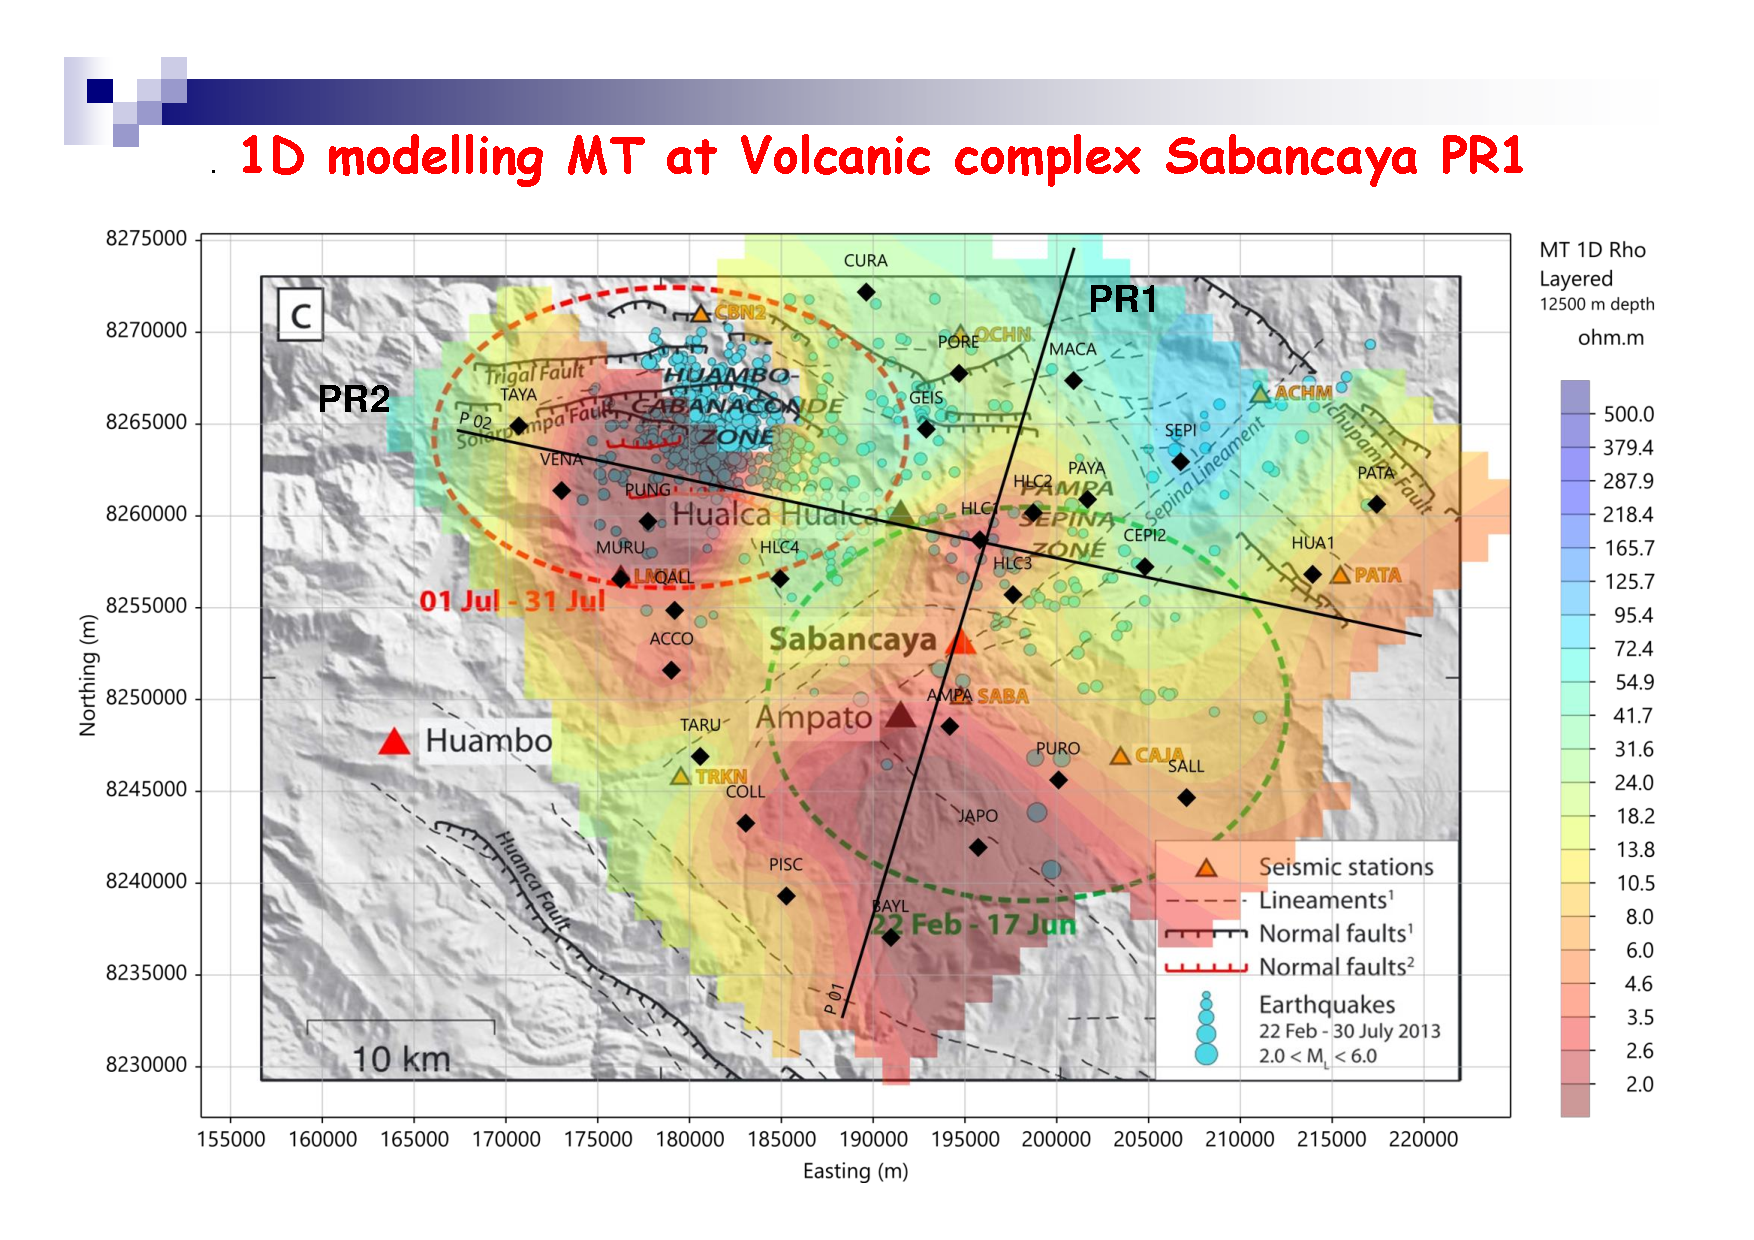
\includepdf[pages=1]{images/MT-2.pdf}
}

{
\setbeamercolor{background canvas}{bg=}
\includepdf[pages=1]{images/MT-3.pdf}
}

{
\setbeamercolor{background canvas}{bg=}
\includepdf[pages=1]{images/MT-4.pdf}
}


\section{Work by R. Machacca \& P. Lesage \\ (Volcanology Team) }

\begin{frame}
 {2016-2017 Seismicity \& Volcanism}
 
 \centering
 \vskip -0.2cm \includegraphics[width=0.9\linewidth]{images/Roger-1.pdf} \\
 
 \hfill \small Machacca et al. (2023)
  
\end{frame}


\begin{frame}
 {2019 Seismicity \& Volcanism}

 \centering
 \vskip -0.2cm  \includegraphics[width=0.9\linewidth]{images/Roger-2.pdf}  \\
\hfill \small Machacca et al. (2023)
 
\end{frame}

\begin{frame}
 
 \centering
 \LARGE Thanks for listening \\
 
 
\end{frame}


\end{document}

